\documentclass{article}
% \twocolumn

\usepackage[round]{natbib}
\usepackage{geometry}
\usepackage{amsmath, amsfonts, amsthm}
\usepackage{algorithm, algpseudocode}
\usepackage{graphicx, subcaption, float}

\graphicspath{{./images/}}

\newcommand{\tskit}{{\texttt{tskit}}}
\newcommand{\tsinfer}{{\texttt{tsinfer}}}
\newcommand{\msprime}{{\texttt{msprime}}}
\newcommand{\twisst}{{\textit{TWISST}}}

\begin{document}

\title{Efficiently Computing Species Trees Distributions Along the Genome}
\author{Daniel Goldstein}
\maketitle


\section{Introduction}

The inference of species trees from genomic data is a fundamental problem in
evolutionary biology. They reveal the relatedness between species and broaden 
our understanding of evolutionary processes. However, there is not generally
only one species tree that can describe a set of samples.
Processes like admixture can create genetic sequences that reflect
alternate species trees.
Genetic events like recombination can cause different regions of the genome
to reflect different species histories within the same sample.
So instead of a single species tree we must consider a distribution
of likelihoods over all possible topologies for every position on the genome.
Inferring these distributions from variant data often requires complex
statistical models and are expensive to compute across large sequences.
Here, we discuss a simple approach for computing exact
species tree distributions that relies on the tree sequence data model.
Using tree sequences, we can compute these results in record time and
scale well in terms of sample size and sequence length.

Tree sequences are a lossless, efficient method of storing and processing
variant data that leverages the shared genetic material between samples.
Samples are represented as leaves in ancestral trees that span
particular intervals of the genome. The high correlation between adjacent
trees in the sequence allows us to store the minimal information to transform
one tree into the next, instead of storing each tree independently. This
significantly decreases storage space and yields an efficient way to iterate
through the data. Using this form iteration, we can design tree sequence
algorithms to recompute only the necessary information required to calculate
the result for the following tree.
This approach is called an incremental algorithm and is the reason this
we can quickly compute species trees distributions for tens of thousands of
trees along the genome.

* This needs many citations

\section{Method}
\subsection{Ranking tree topologies}

Before we can discuss the algorithm for calculating species trees, we
need a system to refer to and identify them uniquely.
In the context of this method, we require that species trees be rooted,
leaf-labelled trees with no unary nodes.
Since there exists a finite number of topologies under this definition
of equality, we can use a combinatorial approach to index, or rank,
tree topologies.
This rank serves as a reversible hash on species trees, meaning we can
easily convert back and forth between a tree representation and its
rank among all possible species trees. The rank is used in the following
algorithms to count occurences of unique species tree topologies.

\subsection{Species trees distributions on a single tree}

The method for computing species trees distributions is inspired by
\twisst{}~\citep{Martin429}, which works
by repetitively selecting samples, one from each species, and tracing the
embedded tree that they form within the larger gene tree.
We can identify the species tree topology supported by that single sample
combination by taking each sample to represent the species from which it
was chosen.
Tallying the number of sample combinations that
reflect each unique topology yields a distribution of species trees
embedded in the single gene tree. By exhausting all sample combinations,
we obtain an exact distribution.

However, this approach scales poorly with sample size as the number
of sample combinations for $n$ samples and $p$ populations is $O(n^p)$ for
$p \ll n$. Approximations can be obtained by running a set number of iterations
but at the cost of needing to choose a fair subset of sample combinations and
accounting for this approximation downstream.

Our method uses a dynamic programming approach to reduce the algorithmic
complexity to be linear in $n$, while also producing an exact distribution.
The approach relies on the following points:
\begin{enumerate}
    % What is the name of a leaf root?
    \item A leaf root contains a single species tree: that of the species to
        which the sample belongs.
    \item An internal node contains the species trees of its children, as
        well as all combinations of trees from its children whose
        sets of species are disjoint.
\end{enumerate}
These rules yield a single-pass algorithm from the leaves of the tree
up to the root. Figure~\ref{fig:dp_alg} and Algorithm~\ref{alg:dp_alg}
illustrate this in the case of binary trees, but the same approach generalizes
to trees with any number of polytomies.

\begin{figure}[H]
    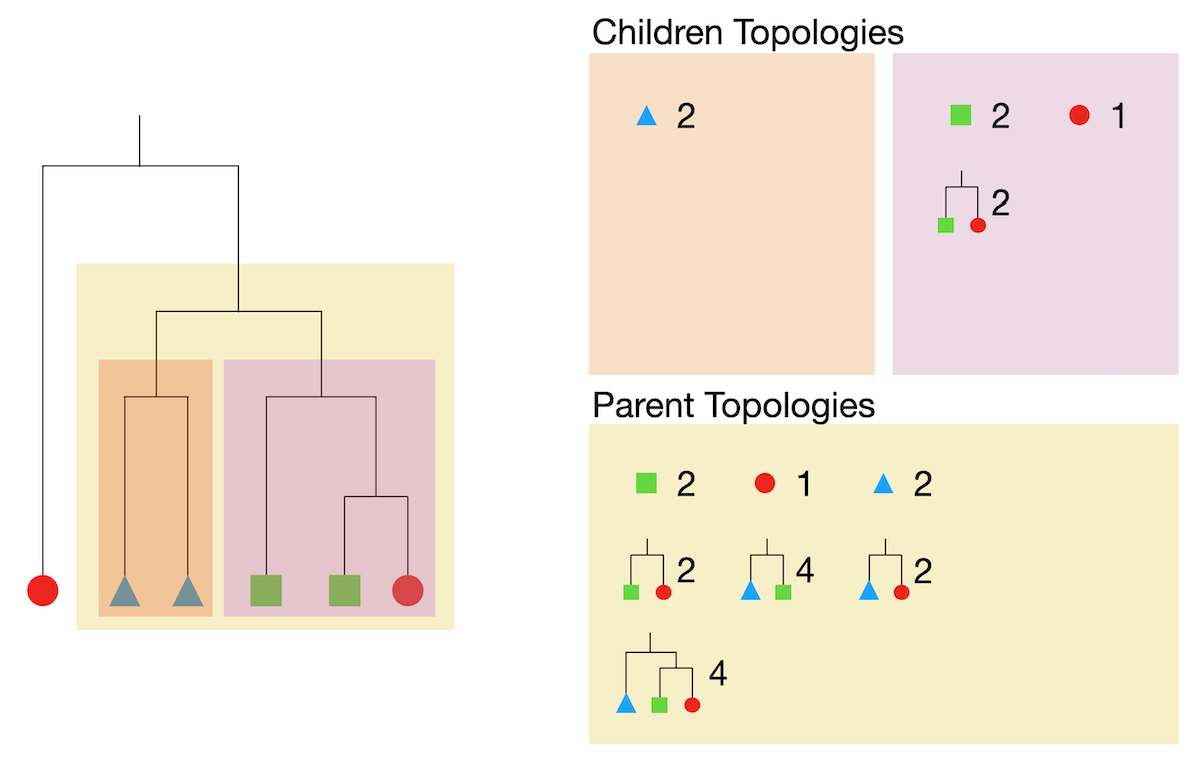
\includegraphics[scale=0.5]{dp_alg}
    \centering
    \caption{Counting embedded species trees at an internal node}
    \label{fig:dp_alg}
\end{figure}

The algorithm state at each node is the unique topologies beneath that node,
represented by their ranks, and the
counts of how many times each topology is represented in the subtree. This
limits the size of the state to the number of unique species tree topologies,
not the number of samples. At an internal node $u$, we perform a cartesian
product of the states of $u$'s children to discover disjoint species trees that
can be combined under $u$.

\begin{algorithm}
    \caption{Computing species tree topologies in a single gene tree}
    \label{alg:dp_alg}
    \begin{algorithmic}
        \State state = []

        \ForAll{$u$ in leaves}
        \State state[$u$] $\leftarrow$ \{(species(u)): 0\} // The rank of a root leaf is 0
        \EndFor

        \ForAll{$u$ in postorder internal nodes}
            \State topologies = \{\}
            \State topologies $\leftarrow$ propagate child topologies // TODO
            \State topologies $\leftarrow$ join disjoint child topologies // TODO
            \State state[$u$] = topologies
        \EndFor
        \State \Return state[root]
    \end{algorithmic}
\end{algorithm}
If we let $t(p)$ be the number of unique tree topologies with $p$ leaves,
we get that the algorithmic complexity is
\[
    O(n \big(\sum_{i=1}^p t(i)\big)^2) = O(n t(p)^2)
\]
since $t(p)$ grows factorially in $p$. We know however that $p \ll n$, so is
dominated by a runtime linear in $n$.

This algorithm also has the nice property that it works on gene trees
that have not completely coalesced. Instead of the final result being
\texttt{state[root]}, we simply take the union of the topology distributions
from each root.

\subsection{Spanning a genome}
This algorithm works well for a single tree, but does not scale when multiplied
across tens or hundreds of thousands of trees as is typical in a tree sequence.
Fortunately, the substructure property allows us to reuse state between trees
where the subtree under a node is unaffected by a tree transition.
As we transition from one tree to the next, instead of constructing
the next tree from scratch we perform a Subtree-Prune-and-Regraft (SPR) operation
on the current tree to obtain the next.
When a node $u$ is removed or inserted into the tree during an SPR, we do not
need to compute the topologies within the subtree.
Instead we need only ``pick up'' the previous algorithm at $u$ and traverse
upward toward the root.
Since there is a constant number of edges removed and inserted between trees
in a tree sequence, this process takes only $O(\log(n)t(p)^2)$ time.
% TODO This could probably be expanded on

\section{Results}
We test this functionality by examining a \msprime{}~\citep{msprime} simulation of four species:
orangutan, gorilla, chimp and human. The simulation was seeded with the underlying
species trees represented in Newick form as: (orangutan, (gorilla, (human, chimp))).
Sampling 1 million 1mb genomes distributed evenly among the four species
produced a \tskit{} tree sequence with 43 thousand trees.
Figure~\ref{fig:great_apes} illustrates the four unique
species tree topologies represented in the tree sequence, the positions
along the sequence they were observed, and the frequency of each weighted by
the length of the sequence they span.

\begin{figure}[H]
    \begin{minipage}{.48\textwidth}
        \begin{subfigure}{\linewidth}
            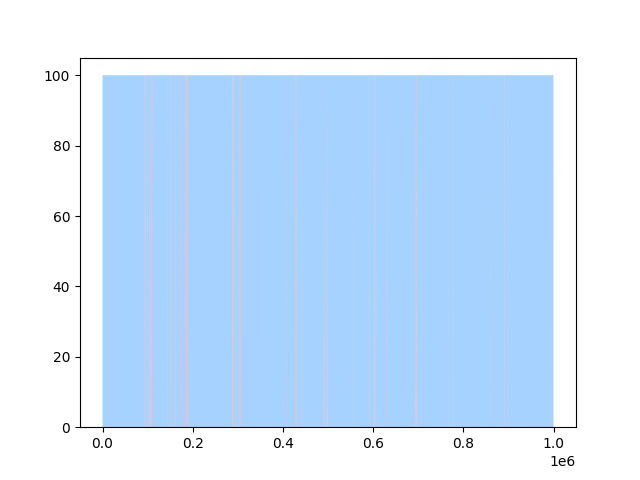
\includegraphics[scale=0.48]{great_apes_area_plot.png}
            \subcaption{Topology frequency per sequence position}
        \end{subfigure}
    \end{minipage}
    \begin{minipage}{.48\textwidth}
        \begin{minipage}{.4\textwidth}
            \begin{subfigure}[b]{\linewidth}
                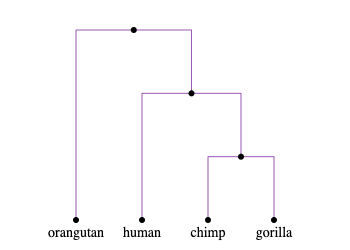
\includegraphics[scale=0.3]{tree_0.png}
                \subcaption{1.85\% weighted}
            \end{subfigure}
            \begin{subfigure}[b]{\linewidth}
                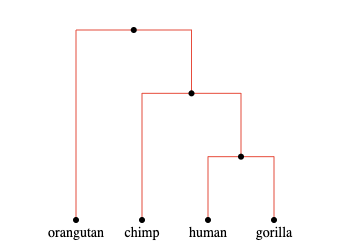
\includegraphics[scale=0.3]{tree_1.png}
                \subcaption{1.67\% weighted}
            \end{subfigure}
        \end{minipage}
        \begin{minipage}{.4\textwidth}
            \begin{subfigure}[b]{\linewidth}
                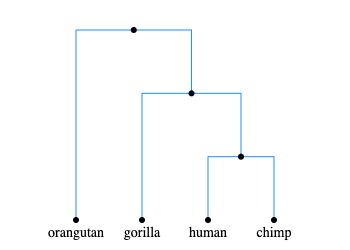
\includegraphics[scale=0.3]{tree_2.png}
                \subcaption{96.43\% weighted}
            \end{subfigure}
            \begin{subfigure}[b]{\linewidth}
                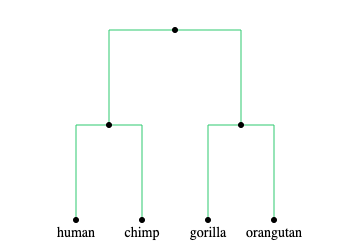
\includegraphics[scale=0.3]{tree_3.png}
                \subcaption{0.06\% weighted}
            \end{subfigure}
        \end{minipage}
        \centering
    \end{minipage}
    \centering
    \caption{Great apes simulated species trees along the genome}
    \label{fig:great_apes}
\end{figure}

The results are greatly aligned with the species tree that seeded the
simulation. Though there do exist three alternative topologies, where the
genetic material coalesces differently. Figure~\ref{fig:great_apes}a presents
the genomic intervals that reflect these anomalous topologies since the algorithm
provides per-tree granularity.

The performance benefits of using an incremental approach is evident when
examining the execution time per tree. Figure~\ref{fig:incremental_times}
show the per-tree wall time and the rate of trees processed per second
for the great apes simulation.
\begin{figure}[H]
    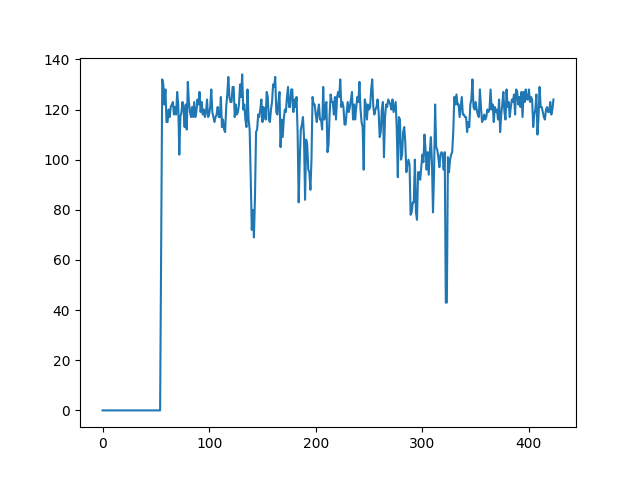
\includegraphics[height=6cm]{trees_per_sec.png}
    \centering
    \caption{Trees processed per second for great apes simulation}
    \label{fig:incremental_times}
\end{figure}

The process described in Algorithm~\ref{alg:dp_alg}
took nearly a minute to compute the distribution of species trees for the first tree.
At this rate, it would take nearly 30 days to process the entire tree sequence if
each tree were considered independently and in serial.
With the incremental algorithm, however, only partial applications of the algorithm
must be made to update the per-node species topologies in subsequent trees, allowing
\tskit{} to process roughly 110 trees per second resulting in an overall
runtime of 7 minutes and 8 seconds. Both the simulation and species tree analysis
were run on a 2015 MacBook Pro with 8GB of RAM.

This simulation portrays an optimal use case for this algorithm. With the tree
sequence being nearly monophyletic, the $p$ term in the algorithm complexity is
nearly nothing. Tree sequences with much more intra-species diversity will express
more species tree topologies and inflate the algorithm state. But ultimately this
overhead is limited by the number of species, $p$, and not by sample size, so will
dominate performance. The combinatorial method of ranking
species trees works elegantly in these use cases where $p$ is small and therefore has
a negligible contribution to the overall runtime. Analyses with larger numbers of
species may benefit from a more efficient indexing mechanism.

Additionally, higher correlation between adjacent trees implies
better gains from using an incremental approach. Current inference methods
like \tsinfer{}~\citep{tsinfer} can generate succinct tree sequences from variant data,
but might not achieve the compression factor of simulated tree sequences and thus
are slower to compute on. Nevertheless, improvements in inference technology have
a compounding effect as tree sequences become more compressed and more accurate,
making incremental algorithms such as this faster and more insightful.

\section{Discussion}


\bibliographystyle{plainnat}
\bibliography{topologies}
\end{document}
